\documentclass[10pt,a4paper]{book}
\usepackage[utf8]{inputenc}
\usepackage{amsmath}
\usepackage{amsthm}
\usepackage{amsfonts}
\usepackage{amssymb}
\usepackage{geometry}
\usepackage{graphicx}
\usepackage{enumitem}
\author{Nicolò Fornari}
\title{Network security}
\newtheorem{remark}{Remark}
\begin{document}
\maketitle
\chapter{Network protocols}
\section{Introduction}
\textbf{Data link layer}\\
It is the lowest logical level, the data link interconnects physical interfaces. Each interface is identified by a MAC address (Media Access Control).\\
The MAC address is 48 bit long, it is usually represented in Hex notation and it is used to route packets in local networks.\\
It uniquely identifies a network interface. It is assigned by the producer according to the standard IEEE 802.\\\\
\textbf{Network Layer}\\
IP operates at this level. IP addresses are dynamically assigned by an authority (eg. ISP's DHCP server).\\\\
\textbf{Stateful:} communication starts, develops,ends. eg. TCP\\
\textbf{Stateless:} IP\\
\newpage
\section{ARP}
ARP (address resolution protocol) allows systems to associate an ip address to a MAC address.\\
All addresses in the ARP table are added by one of these mechanisms:
\begin{itemize}
\item ARP request-reply: \\
who	is	192.168.0.16 tell 192.168.0.1\\
192.168.0.16	is	at	00-10-BC-2c-11-56
\item Gratuitous ARP\\
192.168.0.16	is	at	00-10-BC-2c-11-56
\end{itemize}
\textbf{ARP frame header}\\\\
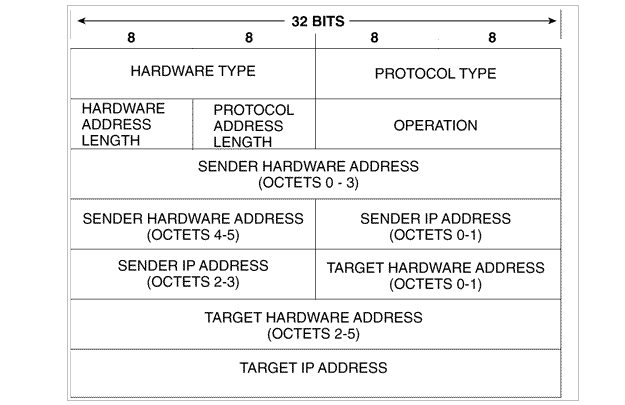
\includegraphics[scale=0.6]{arp.png}\\
\textbf{ARP poisoning}\\
The ARP protocol is declarative, it does not need an answer.\\
Nodes are not authenticated.\\
Limitations: it works only on LAN\\\\
\newpage
\textbf{Subnets and CIDR}\\
Subnets are logical divisions of IP addresses. IP bits are partitioned as network,subnet,host.\\
A subnet mask indicates sections of IP addresses meant for network and subnet.\\
Eg. 255.255.255.0 means 24 bits for network and subnet and 8 bits for hosts.\\\\
\textbf{CIDR}\\
Classless Inter Domain Routing, it is a synthetic way to represent subnet masks.\\
\emph{Example: }
\begin{itemize}
\item Network mask: 255.255.0.0.
\item CIDR representation: 132.132.1.10/16
\item Hosts = $2^{16}$
\end{itemize}
\emph{Formulas:} (everything as binary)
\begin{itemize}
\item Network = Ip AND Subnet
\item Host = Ip AND Not(Subnet)
\end{itemize}
\newpage
\section{IP}
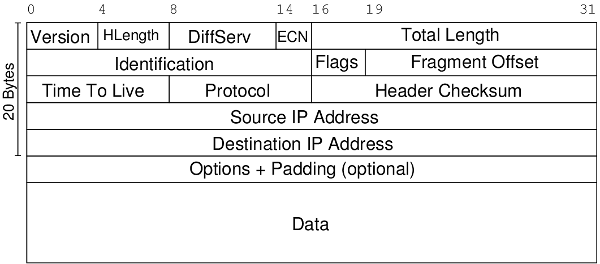
\includegraphics[scale=0.5]{ip.png}\\
Some IPs are reserved for private networks:
\begin{itemize}
\item 10.0.0.0 $\to$ 10.255.255.255
\item 192.168.1.1 $\to$ 192.168.255.255
\item 172.16.0.0 $\to$ 172.16.255.255
\end{itemize}
\textbf{Def} A \emph{datagram} is a basic transfer unit associated with a packet-switched network. The delivery, arrival time, and order of arrival need not be guaranteed by the network.\\\\
\textbf{Def} MTU maximum transmission unit\\\\
\textbf{IP fragmentation}
\emph{Identification:} 16 bit, is the unique identifier of the fragmented datagram.\\
Note that all fragments have the same identification number.\\
\emph{Flags:} 3 bits
\begin{itemize}
\item 0 Reserved, must be zero
\item DF Don't fragment\\
If set to 0 $\to$ there may be fragments\\
If set to 1 $\to$ drop datagram if it has to be fragmented
\item MF More fragments\\
0 $\to$ last fragment\\
1 $\to$ there are more fragments
\end{itemize}
\emph{Offset} 13 bits, offset of this datagram wrt the first fragment with that ID
\newpage
\textbf{Fragmentation example}\\\\
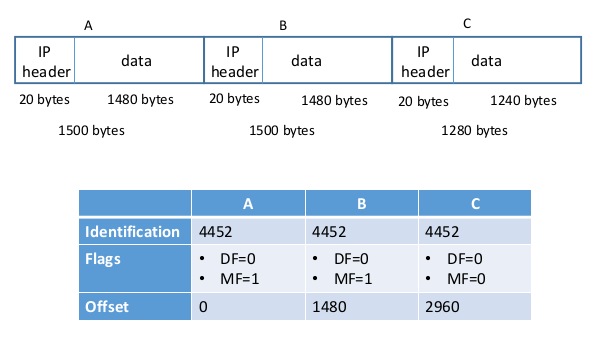
\includegraphics[scale=0.6]{fragmentation.png}\\
\begin{remark}
\textbf{DOS with IP fragments}
You keep sending fragments without sending the first fragment, the router keeps waiting for it until it exhausts its memory.
\end{remark}
\newpage
\section{ICMP} Internet control message protocol. It relies on IP and is and integral part of it.\\\\
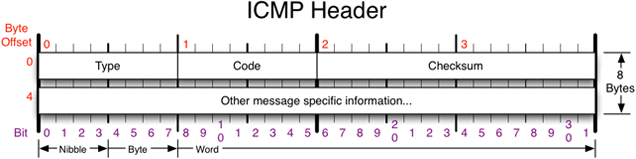
\includegraphics[scale=0.9]{icmp.png}\\\\
\textbf{Some message types}
\begin{itemize}
\item 0		Echo Reply
\item 3		Destination	Unreachable\\
Code 0 $\to$ Net unreachable\\
Code 1 $\to$ Host unreachable\\
Code 2 $\to$ Protocol unreachable\\
Code 3 $\to$ Port unreachable\\
Code 4 $\to$ Fragmentation needed and DF set\\
Code 5 $\to$ Source route failed
\item 4		Source	Quench
\item 5		Redirect
\item 8		Echo
\item 11		Time Exceeded\\
Code 0 $\to$ Net unreachable\\
Code 1 $\to$ Host unreachable
\item 12		Parameter Problem
\item 13		Timestamp
\item 14		Timestamp Reply
\item 15		Information	Request
\item 16		Information	Reply
\end{itemize}
\section{Traceroute}
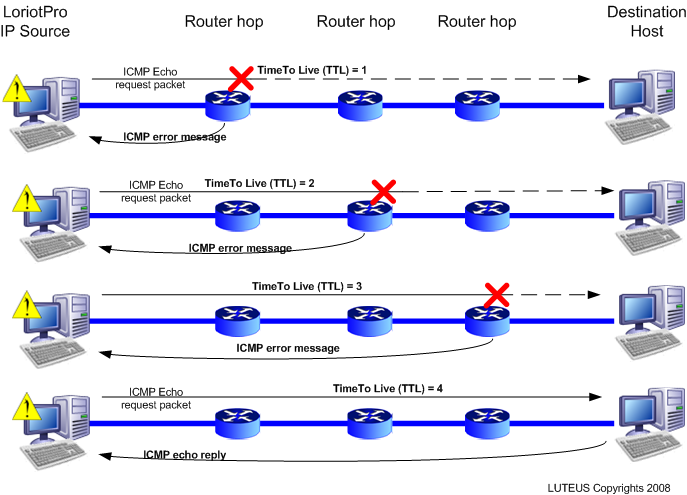
\includegraphics[scale=0.5]{traceroute.png}
\newpage
\section{Denial of service}
\textbf{Def} a Denial of Service is a type of attack that aims at congesting or overpowering a system's capacity by generating requests the system will have to answer.\\\\
\textbf{Examples}
\begin{itemize}
\item Dos with IP fragmentation
\item Ping Flooding (the attacker exploit his wider bandwidth)
\item Ping of death
\end{itemize}
\chapter{Osi Transport Layer}
\section{TCP}
The Transmission Control Protocol builds on top of IP the notion of state. Infact IP just delivers data while TCP manages the data segments by mean of checksums and re-delivery of unreceived/corrupted packets.\\
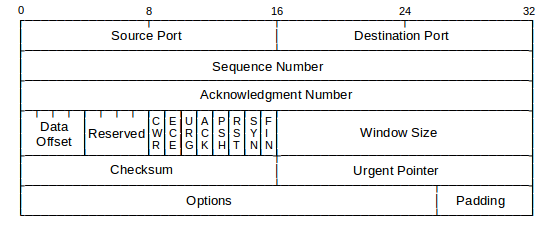
\includegraphics[scale=0.8]{tcp-header.png}\\
A server and a client that partecipate in a TCP connection open a \emph{socket} which is a tuple (source-ip:source-port,destination-ip:destionation-port).\\
Note that a client generates a source port randomly.\\
\textbf{TCP details - some flags:}
\begin{itemize}
\item \textbf{SYN:} initializes the TCP session, it should be set to 1 only for the first datagram
\item \textbf{ACK:} ackwnoledge the reception of the segment
\item \textbf{FIN:} it signals the intention of closing the connection
\item \textbf{RST:} drop the connection (reset)
\end{itemize}
\textbf{Sequence number:} it is a 32 bit generated by each end (note that the sequence number of the client is independent from the server's one).\\
\textbf{Acknoledgement number:} 32 bits\\\\
\newpage
\section{Handshakes}
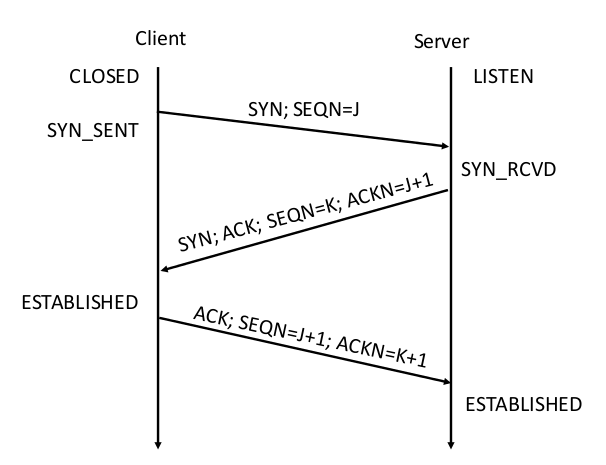
\includegraphics[scale=0.5]{3-way.png}\\\\
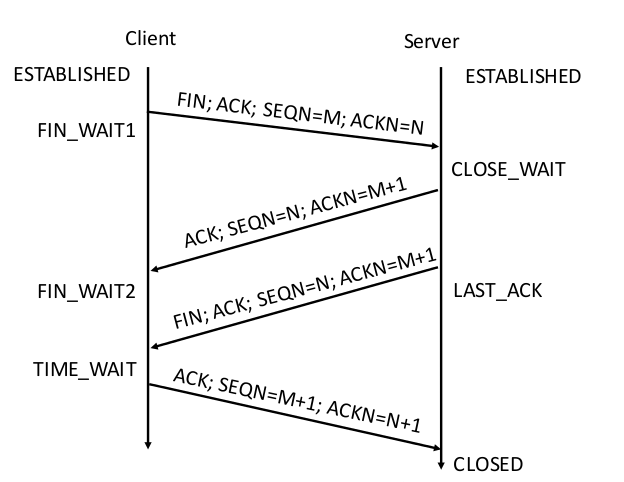
\includegraphics[scale=0.5]{4-way.png}
\newpage
\section{Some TCP specifics}
Both client and server set up a TCB (Transmission control block) to keep track of connection. The TCB structure is freed from memory when connection reaches status CLOSED.\\\\
A packet with RST flag up does not receive an answer.\\
If the state is CLOSED any packet with no RST receives a RST.\\
If the state is LISTEN 
\begin{itemize}
\item SYN flag up + no ACK opens a TCP session. Answer is SYN+ACK
\item Only ACK receives a RST
\item Drop with no answer otherwise
\end{itemize}
\section{SYN DoS}
When the server receives SYN J it answers back with SYN K, ACK J+1.\\
The server opens a new session in a separate threat/ allocates resources. Then the server waits for the ACK K+1 from the client, it waits for the MSL (maximum segment lifetime set by default to 2 minutes). The same mechanism is on the sender side but of course the attacker controls it and can bypass it.\\\\
The attacker drops all SYN ACKs with a firewall to avoid exhausting its own resources. Note that a server typically has more bandwidth than a single client.
\begin{remark}
The attack currently works in $\mathcal{O}(2n)$ because for each SYN a SYN ACK is received $\to$ less bandwidth.
\end{remark}
However the attack can be improved by spoofing the source ip address, now the attacker is operating in $\mathcal{O}(n)$.\\
In theory the attack should not work because the server should receive a RST by each zombie, consequently free the TCB making the attack fail.\\
Still the attacker can choose a set of IPs which do not reply.
\section{Dos mitigations}
\begin{itemize}
\item Load balancing: distribute traffic loads evenly
\item Rate limiter: deny traffic above a certain rate of SYN/sec
\item Proof of work: require the source to solve a cryptopuzzle before allocating resources for the connection (note that this requires a protocol support).
\end{itemize}
\newpage
\section{TCP scans}
It is possible to exploit specifications of a network protocol (TCP,UDP,..) to learn something about a system or a network.\\\\
\textbf{SYN Scan:} the attacker forges TCP packets with SYN=1. It is useful to see whether the remote system accepts incoming connections on a certain port.\\
Note that a polite way of scanning is performed in the following way: after the server's SYN ACK reply, the attacker sends a RST so that the 3-way handshake is never finished.\\\\
\textbf{Host fingerprinting:} different operating systems have their own independent implementation of the TCP stack.\\\\
\textbf{Examples:}
\begin{itemize}
\item FIN = 1
\item all flags set to 0
\item Xmas: FIN,URG,PSH = 1
\end{itemize}
\newpage
\section{TCP Session hijacking - Mitnick attack}
The attacker wants to send commands to a server they have no access to (eg. simple IP address authentication). The server has to think the attacker is the client, however the attacker does not sit in between client and server.\\\\
A TCP segment is identified and validated by:
\begin{itemize}
\item client ip $\to$ known
\item destination ip $\to$ known
\item port $\to$ known (if not standard, scan)
\item client SEQ number $\to$ known(the attacker generates it)
\item server SEQ number $\to$ \emph{unknown}
\end{itemize}
Back in the old days algorithms for generating the SEQ number were really simple.\\\\
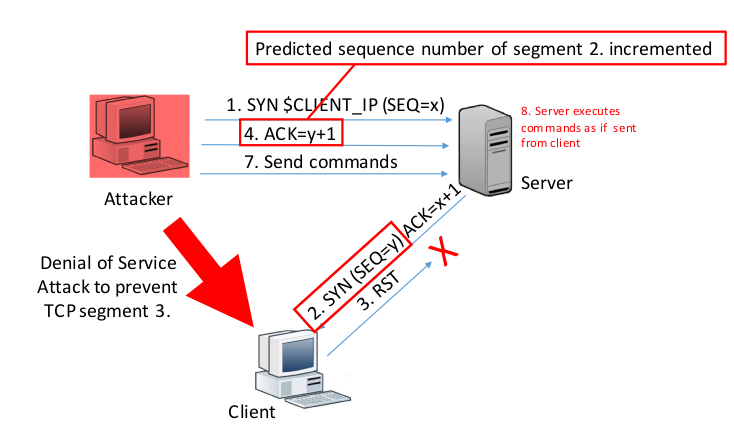
\includegraphics[scale=0.6]{mitnick-attack.png}
\newpage
\section{UDP}
The User Datagram protocol is a stateless. It is designed for fast delivery of data
\begin{itemize}
\item Data integrity can be controlloed at application level
\item It relies on the reliability of the underlying network link
\item It does not guarantee delivery (there is no ACK mechanism)
\end{itemize}
\textbf{Usage}
\begin{itemize}
\item DNS servers
\item NFS (network file systems)
\item SNMP (simple network management protocol)
\item DHCP (dinamic host configuration protocol)
\item Most real time applications
\end{itemize}
\section{UDP scans}
It can be used to discover open ports on the network:
\begin{itemize}
\item CLOSE $\to$ ICMP port unreachable
\item OPEN $\to$ no answer
\end{itemize}
However it is possible to configure a stealth system that does not reply to UDP requests to CLOSED ports by dropping ICMP packets with a firewall or router.
\chapter{Osi Session - Presentation - Application Layer}
\section{DNS}
DNS (Domain Name Service) is a hierarchical system for domain name resolving. It translates human readable addresses to IP addresses the domain is reachable at. It uses UDP for fast answer (port 53).\\
\textbf{Motivation:} it is possible to assign multiple names to the same ip or viceversa. This flexibility is useful for:
\begin{itemize}[noitemsep,nolistsep]
\item Server substitution
\item Virtual hosting (a single server hosting multiple websites)
\item A name is assigned to multiple IPs (so that the workload is distributed).
\end{itemize}
There exists different kind of DNS records, here we lista few:
\begin{itemize}[noitemsep,nolistsep]
\item \textbf{A} correspondence name - IP(s)
\item \textbf{AAAA} Same as A but works for ipv6
\item \textbf{NS} ip of the DNS server to ask
\end{itemize}
\textbf{DNS hierarchy}
\begin{itemize}[noitemsep,nolistsep]
\item Root DNSs $\to$ they are responsible for top level domain queries
\item Authoritative DNS $\to$ A DNS that "knows the answer" (ie. it does not ask to other DNSs)
\item Recursive DNS $\to$ It forwards queries to authoritative DNSs
\end{itemize}
\subsection{DNS Cache poisoning}
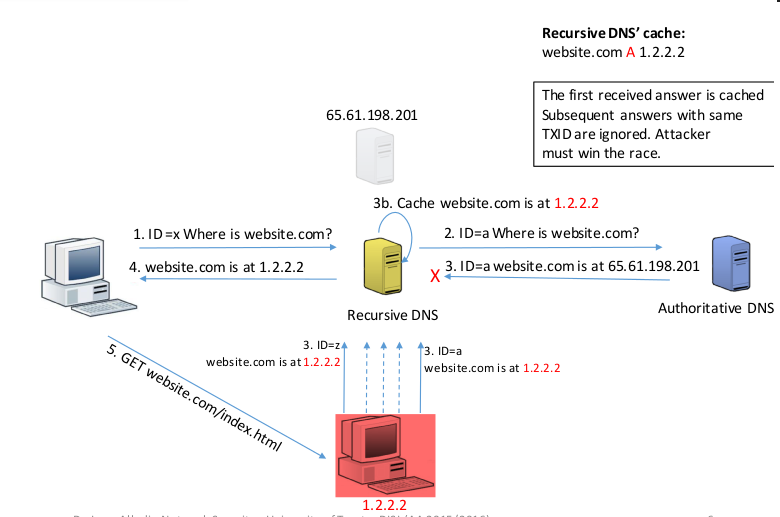
\includegraphics[scale=0.6]{dns-poisoning.png}
\newpage
\subsection{Kaminsky attack}
The attacker rather than replacing an A record replaces an NS record, in this way he can get control over any (sub)domain.\\
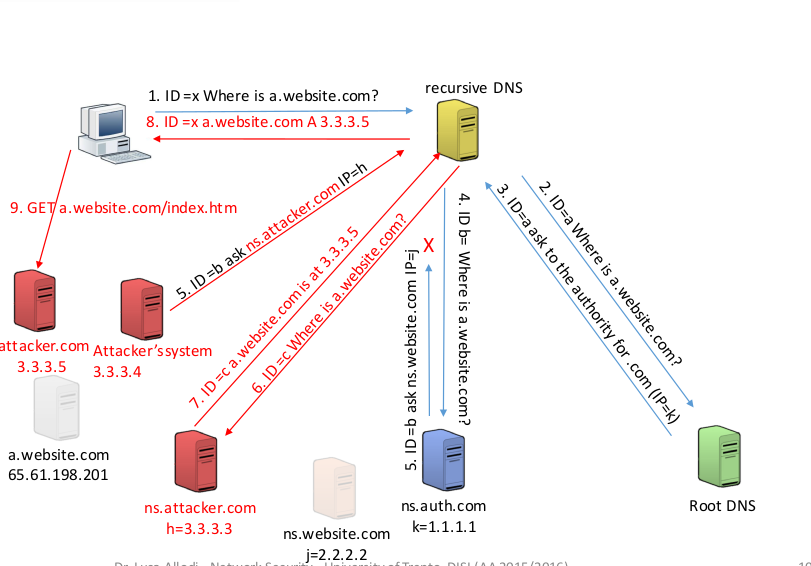
\includegraphics[scale=0.6]{kaminsky-attack.png}\\
\textbf{Mitigation:} the source of attack is low entropy with a 16 bit ID. Randomness is not enough and it is not feasible to change the protocol to 32 bits. \\
The solution is to randomize the source port to increase the entropy: any answer that does not match both source port and transaction ID will be dropped.
\newpage
\subsection{DNS amplification attack}
It is DoS attack that exploits certain types of DNS answers that are much bigger in size than the requests.\\
Recall that the DNS works over UDP so the source IP is easy to spoof.
\subsection{DNS zone transfer}
A sone is a domain for which a server is authoritative. "Slave" servers can ask "authoritative" servers to copy their zone database (over TCP).\\
An attacker pretends to be a slave server and dump the zone DB. In this way he acquires knowledge of zone's infrastructure and it is eased in performing further attacks.
\subsection{DNS Sec}
It is a secure implementation of the DNS protocol: it implements DNS auth on top of normal DNS. Note that it protects just integrity and not confidentiality.
\section{HTTP}
HTTP is the main protocol on which the www works. It is based on the notion that a client can either reuest or submit data to a server. There are two methods: GET and POST.\\
HTTP is stateless, HTTP cookies enable statefulness.
\subsection{Cookies}
\begin{itemize}
\item Domain  (who can read)
\item Expires (if NULL valid only for a session)
\item Secure (only over SSL)
\end{itemize}
\textbf{HTTP session hijacking} the attacker can read the session ID cookie and spoof the victim's identity (eg. facebook until 2011).\\
Secure cookies provide confidentiality but no integrity.
\section{Telnet}
It is a protocol used in remote control services. It operates over TCP port 23. Typically there is no authentication and no encryption.
\section{Common issues}
\begin{itemize}
\item Lack of authentication
\item Communication channel is in the clear
\end{itemize}
\chapter{Vulnerabilities}
\textbf{Software bug} a bug is a problem in the execution of the software that leads to unexpected behaviour (eg. crashes,infinite loops, wrong entries of db displayed)\\
Charachteristics of a bug
\begin{itemize}
\item Replicability
\item Logic/configuration/design/implementation
\item Fix priority
\item If it is documented it is a feature
\end{itemize}
\section{Types of vulnerabilities}
\begin{itemize}
\item Configuration v.\\
eg. Ssh accepts root connections from any ip
\item Insfrastructural v.\\
eg. sensitive db in a network's DMZ
\item Software v.\\
eg. authorization mechanism can be bypassed
\end{itemize}
\section{Vulnerability discovery}
Vulnerabilities are different in nature
\begin{itemize}
\item Often implementation dependent
\item May require deep understanding of sw module interaction
\item Necessary in-depth knowledge of system design (kernel structure, memory allocation)
\end{itemize}
Discovery techniques
\begin{itemize}
\item Code lookups (searches for known patterns)\\
either you are a developer or the software is open source
\item Fuzzing (semi-automatic random input generation)
\item Google hacking (outdated)\\
you look for software that you already know it is vulnerable
\end{itemize}
Vulnerabilites can be found either internally or externally to a company.\\
\section{Vulnerability handling}
The ISO 30111 is a standard to handle vulnerabilities.\\
\textbf{The initial investigation}
\begin{itemize}
\item The reported problem is a security vulnerability
\item The vulnerability affects a supported version of the software the vendors maintains, not third parties modules (else: exit).
\item The vulnerability is eploitable with know techniwues (else: exit)
\item Root cause analysis
\item Prioritisation (evaluate potential threat)
\end{itemize}
\textbf{Resolution decision}\\
Vendor must decide how to resolve the vulnerability.
\begin{itemize}
\item Configuration v. $\to$ advisory may be enough
\item Code v. $\to$ patch
\item Critical v. $\to$ release a mitigation before full patch
\end{itemize}
\textbf{Remediation development}\\
Every solution must be tested before being delivered. This is very expensive both for customer and vendor\\\\
\textbf{Release and Post-Release}\\
\section{Different issues}
Vulnerability advisories are typically published after pathcing.\\
Security researchers expect economic return and or credit.\\
Issue: communication between security researcher and the vendor: tradeoff between saying little and being verbose.\\
Often involves development of Proof of concept exploit to show the vulnerability is exploitable.



\end{document}